\documentclass[11pt,]{article}
\usepackage[left=1in,top=1in,right=1in,bottom=1in]{geometry}
\newcommand*{\authorfont}{\fontfamily{phv}\selectfont}
\usepackage[]{mathpazo}


  \usepackage[T1]{fontenc}
  \usepackage[utf8]{inputenc}



\usepackage{abstract}
\renewcommand{\abstractname}{}    % clear the title
\renewcommand{\absnamepos}{empty} % originally center

\renewenvironment{abstract}
 {{%
    \setlength{\leftmargin}{0mm}
    \setlength{\rightmargin}{\leftmargin}%
  }%
  \relax}
 {\endlist}

\makeatletter
\def\@maketitle{%
  \newpage
%  \null
%  \vskip 2em%
%  \begin{center}%
  \let \footnote \thanks
    {\fontsize{18}{20}\selectfont\raggedright  \setlength{\parindent}{0pt} \@title \par}%
}
%\fi
\makeatother




\setcounter{secnumdepth}{3}

\usepackage{longtable,booktabs}

\usepackage{graphicx,grffile}
\makeatletter
\def\maxwidth{\ifdim\Gin@nat@width>\linewidth\linewidth\else\Gin@nat@width\fi}
\def\maxheight{\ifdim\Gin@nat@height>\textheight\textheight\else\Gin@nat@height\fi}
\makeatother
% Scale images if necessary, so that they will not overflow the page
% margins by default, and it is still possible to overwrite the defaults
% using explicit options in \includegraphics[width, height, ...]{}
\setkeys{Gin}{width=\maxwidth,height=\maxheight,keepaspectratio}

\title{Patrones de Ecología Numérica Descritos por la Familia de Plantas
Fabaceae Mimosoideae en la Isla Barro Colorado, Cuenca del Mar Caribe.\\
\emph{Patterns of Numerical Ecology Described by Plants Family Fabaceae
Mimosoideae in Barro Colorado Island, Caribbean Sea Basin}.\\  }



\author{\Large Welifer Junior Lebron Vicente\vspace{0.05in} \newline\normalsize\emph{Estudiante de Ciencias Geográficas, Universidad Autónoma de Santo
Domingo (UASD)}  }


\date{}

\usepackage{titlesec}

\titleformat*{\section}{\normalsize\bfseries}
\titleformat*{\subsection}{\normalsize\itshape}
\titleformat*{\subsubsection}{\normalsize\itshape}
\titleformat*{\paragraph}{\normalsize\itshape}
\titleformat*{\subparagraph}{\normalsize\itshape}

\titlespacing{\section}
{0pt}{36pt}{0pt}
\titlespacing{\subsection}
{0pt}{36pt}{0pt}
\titlespacing{\subsubsection}
{0pt}{36pt}{0pt}





\newtheorem{hypothesis}{Hypothesis}
\usepackage{setspace}

\makeatletter
\@ifpackageloaded{hyperref}{}{%
\ifxetex
  \PassOptionsToPackage{hyphens}{url}\usepackage[setpagesize=false, % page size defined by xetex
              unicode=false, % unicode breaks when used with xetex
              xetex]{hyperref}
\else
  \PassOptionsToPackage{hyphens}{url}\usepackage[unicode=true]{hyperref}
\fi
}

\@ifpackageloaded{color}{
    \PassOptionsToPackage{usenames,dvipsnames}{color}
}{%
    \usepackage[usenames,dvipsnames]{color}
}
\makeatother
\hypersetup{breaklinks=true,
            bookmarks=true,
            pdfauthor={Welifer Junior Lebron Vicente (Estudiante de Ciencias Geográficas, Universidad Autónoma de Santo
Domingo (UASD))},
             pdfkeywords = {Ecología Numérica, BCI, Análisis Forestal, Lenguaje R},  
            pdftitle={Patrones de Ecología Numérica Descritos por la Familia de Plantas
Fabaceae Mimosoideae en la Isla Barro Colorado, Cuenca del Mar Caribe.\\
\emph{Patterns of Numerical Ecology Described by Plants Family Fabaceae
Mimosoideae in Barro Colorado Island, Caribbean Sea Basin}.\\},
            colorlinks=true,
            citecolor=blue,
            urlcolor=blue,
            linkcolor=magenta,
            pdfborder={0 0 0}}
\urlstyle{same}  % don't use monospace font for urls

% set default figure placement to htbp
\makeatletter
\def\fps@figure{htbp}
\makeatother

\usepackage{pdflscape} \newcommand{\blandscape}{\begin{landscape}}
\newcommand{\elandscape}{\end{landscape}}


% add tightlist ----------
\providecommand{\tightlist}{%
\setlength{\itemsep}{0pt}\setlength{\parskip}{0pt}}

\begin{document}
	
% \pagenumbering{arabic}% resets `page` counter to 1 
%
% \maketitle

{% \usefont{T1}{pnc}{m}{n}
\setlength{\parindent}{0pt}
\thispagestyle{plain}
{\fontsize{18}{20}\selectfont\raggedright 
\maketitle  % title \par  

}

{
   \vskip 13.5pt\relax \normalsize\fontsize{11}{12} 
\textbf{\authorfont Welifer Junior Lebron Vicente} \hskip 15pt \emph{\small Estudiante de Ciencias Geográficas, Universidad Autónoma de Santo
Domingo (UASD)}   

}

}








\begin{abstract}

    \hbox{\vrule height .2pt width 39.14pc}

    \vskip 8.5pt % \small 

\noindent Las fabaceas son plantas de amplia distribución terrestre, sus
características y propiedades las hacen importantes en diversos campos
de la ciencia médica, la industria alimenticia y textil. Los métodos de
análisis biogeográficos permiten cuantificar el estado de esta familia,
brindando información valiosa para comprender las formas de asociación,
agrupamiento, proliferación y decaimiento de acuerdo a variables
ambientales. En la isla Barro Colorado el clado filogenético mimosoide
presente no exhibe comportamientos que favorezcan variables edáficas y
geomorfológicas específicas de manera marcada.


\vskip 8.5pt \noindent \emph{Keywords}: Ecología Numérica, BCI, Análisis Forestal, Lenguaje R \par

    \hbox{\vrule height .2pt width 39.14pc}



\end{abstract}


\vskip 6.5pt


\noindent  \section{Introducción}\label{introducciuxf3n}

El análisis de biodiversidad forestal viabiliza la obtención de
información sobre el comportamiento de las especies en su hábitat, los
efectos de cambios geoestacionarios, y las probables consecuencias de
actividades antrópicas en el ciclo vital de los bosques; cuya función en
el caso de los tropicales puede ser productiva (madera, fibra, leña,
productos no maderables); ambiental (regulación del clima, reserva de
biodiversidad, conservación de suelos y agua, etc.); y social
(subsistencia de poblamientos humanos locales y su cultura) (Montagnini,
Jordan, \& others, 2005).

La isla Barro Colorado (BCI), de coordenadas {[}9º 9' 0'`N, 79º 51' 0''
W{]}, es una plataforma basáltica miocénica sobre la que descansa un
bosque tropical primario compuesto por 305 especies arbóreas (Condit et
al., 1999). Fue el emplazamiento de ocho censos forestales realizados
por el Smithsonian Tropical Research Institute entre 1981 y 2015, donde
la subfamilia \emph{Fabaceae Mimosoideae} representó el 5.9\% de las
especies registradas en la parcela de 50 hectáreas delimitada en 1980.

\begin{figure}
\centering
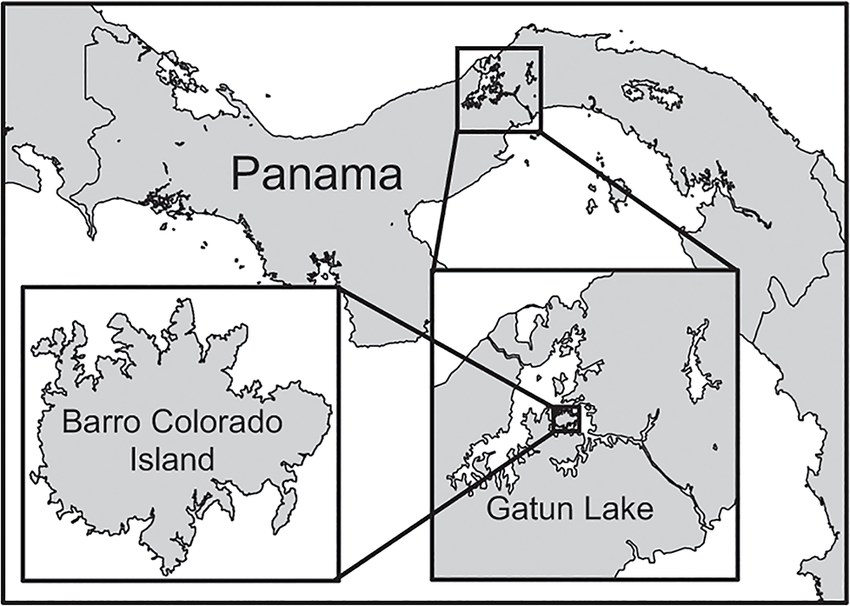
\includegraphics[width=0.50000\textwidth]{Map-of-Barro-Colorado-Island-BCI-Panama.png}
\caption{Isla Barro Colorado, Panamá (Baldeck et al., 2014).}
\end{figure}

El registro forestal de BCI forma parte de una serie de parcelas
permanentes delimitadas en distintas latitudes y longitudes, pero dentro
de la zona tropical. Estas parcelas poseen diferencias climáticas
específicas con el objetivo de contabilizar, supervisar y medir
variables demográficas que viabilicen realizar comparaciones atendiendo
a cuestionamientos científicos, registro detallado del comportamiento en
ecología vegetal o problemáticas resultantes de la intervención humana
en el equilibrio natural (Condit, 1998).

\begin{figure}
\centering
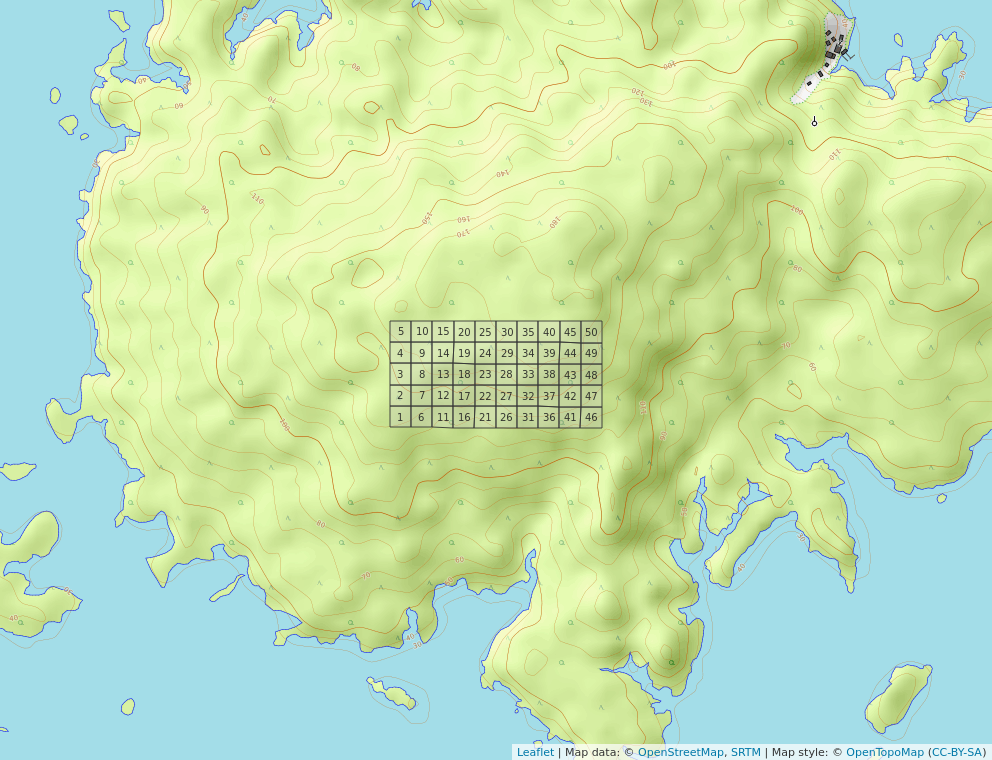
\includegraphics[width=0.50000\textwidth]{mapa_cuadros.png}
\caption{Área del censo forestal, Barro Colorado Island (1981-2015).}
\end{figure}

Las fabaceas concentran su diversidad en la franja tropical y
subtropical, aunque se encuentran ampliamente distribuidas por la
práctica totalidad de climas terrestres. Están presentes en zonas
árticas, litoral costero, ambientes alpinos, bosque lluvioso, bosque
estacional, sabanas, bosque seco, desiertos áridos, pantanos y
manglares. Poseen características especializadas que las hacen vitales
para el equilibrio ecológico y para la supervivencia del ser humano.
Asimismo, el 88\% de las especies de fabaceas pueden formar nódulos con
bacterias (rhizobia) para fijar el N2 en la atmósfera mediante
asociación simbiótica, fisiología rica en proteínas, etc.; mientras que
sus semillas son empleadas para tratar células cancerígenas, sus
componentes químicos las hacen esenciales para diversos tipos de
industrias, y el grano de las leguminosas representa el 33\% del
nitrógeno necesario en la dieta del ser humano (Saikia, Nag, Anurag,
Chatterjee, \& Khan, 2020). Especificando, la subfamilia
\emph{Mimosoideae} dentro del clado filogenético mimosoide es sumamente
variable, estando compuesta principalmente por árboles y arbustos de
flores simétricas cigomorfas con pétalos valvados, a la vez que sus
especímenes tienen un gran número de estambres prominentes
(Hasanuzzaman, Araújo, \& Gill, 2020). En BCI se encuentran 18 de estas
especies.

\begin{figure}
\centering
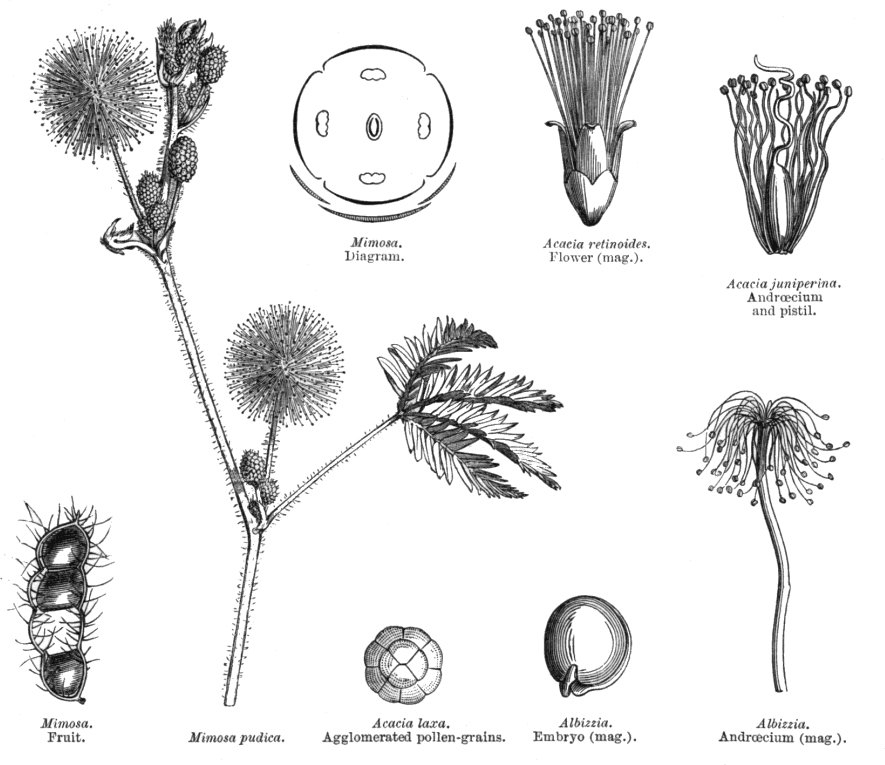
\includegraphics[width=0.50000\textwidth]{Grabado-Mimosoideae.png}
\caption{Grabado de fabaceas (Universiad de Toronto). \label{fig:grab}}
\end{figure}

Atendiendo a la flexibilidad en la distribución de las fabáceas, su
importancia económica, y social; se busca entender qué factores
ambientales intervienen en la proliferación, agrupamiento o decaimiento
de sus poblaciones en bosques tropicales que comparten características
con los hallados en República Dominicana, en esta ocasión tomando la
data cincuentenaria recolectada y provista por The Center for Tropical
Forest Science en BCI. En ese sentido, la ecología numérica es el campo
de estudio que brinda las técnicas, índices, y herramientas necesarias
para obtener conclusiones a partir de data forestal, animal, y biotopo.
R es un software de código abierto y ambiente de programación que brinda
una amplia variedad de facilidades para el manejo, creación, y
visualización gráfica de ciencia de datos, resultando ideal para este
campo de estudio (Venables, Smith, Team, \& others, 2009).

Los métodos de análisis en ecología númerica han incrementado
exponencialmente a partir de la década 1950, desarrollandose índices,
estimadores y algoritmos que permiten realizar transformaciones
cualitativas y cuantitativas para inferir y obtener presición con
menores probabilidades de sesgo o en ausencia del mismo. La obtención de
información relativa al grado de asociación, ordenamiento, diversidad,
agrupamiento, entre otros; es debida a estas técnicas. (ver tabla
\ref {tab:met})

Table 1: Métodos de análisis en ecología numérica empleados (Moreno,
2001).\label{tab:met}
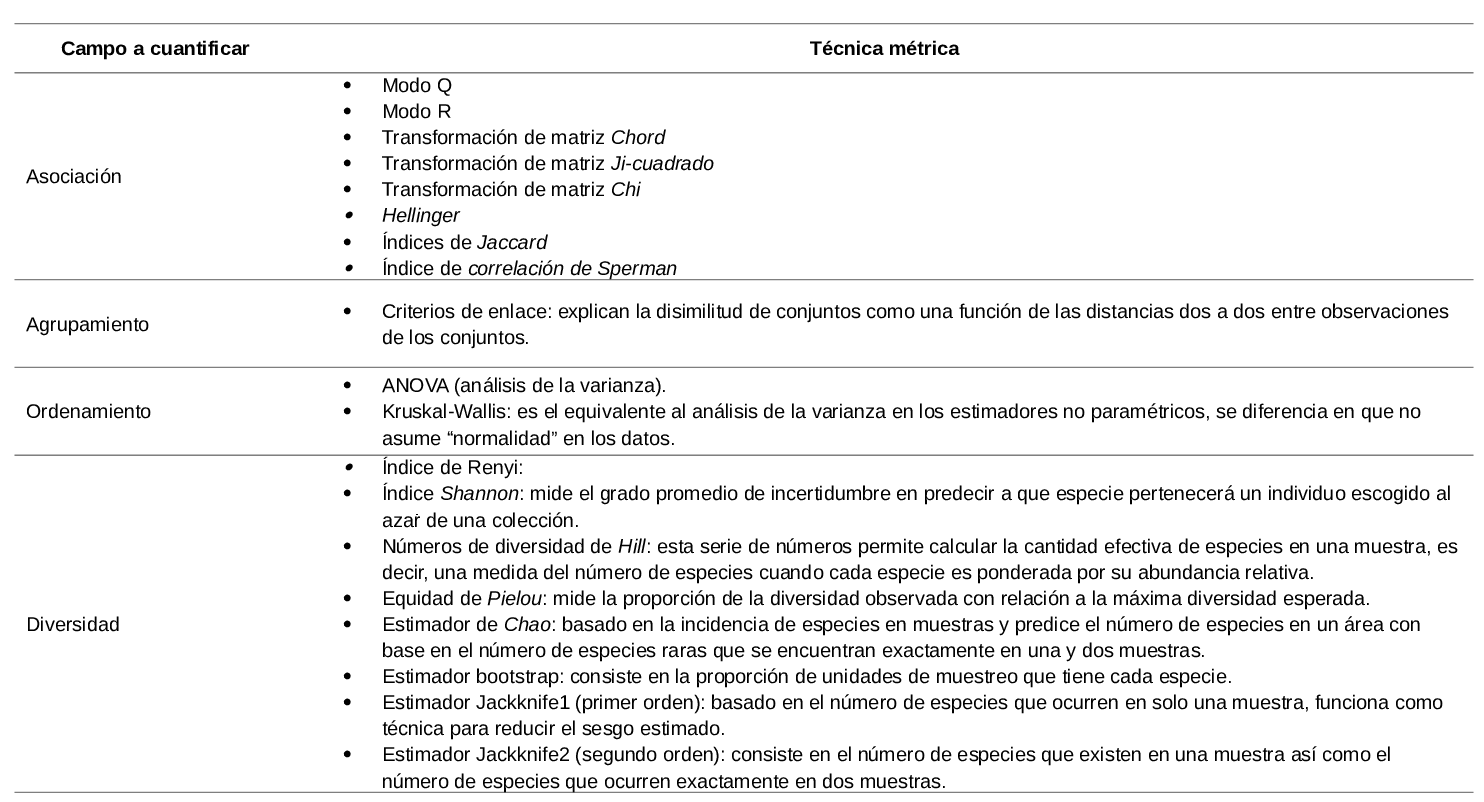
\includegraphics[width=1.00000\textwidth]{Análisis/Diversidad/Tabla_Métodos_Análisis.png}

\ldots

\section{Metodología}\label{metodologuxeda}

Obtenida la data censal de Barro Colorado, se empleó R para realizar
análisis estadísticos, gráficos, matrices, y mapas a la matriz de la
familia \emph{Fabaceae mimosoideae} partiendo del repositorio
\textbf{Scripts de análisis BCI} (Batlle, 2020).

La creación de los utiles necesarios para los análisis fue posible
mediante el empleo de los paquetes \emph{vegan}, \emph{tydiverse}, y
\emph{sf} para extraer la familia \emph{Fabaceae Mimosoideae} de la data
censal, obtener las estadísticas, gráficos lineales y diagramas de
cajas. A la vez que, mediante \emph{mapview} se crearon, proyectaron y
almacenaron los mapas; con \emph{RColorBrewer} se para obtuvo una gama
de colores más amplia en los gráficos y mapas; y con \emph{broom} se
visuaizaron las matrices de distancia. Otros paquetes empleados fueron
\emph{magrittr}, \emph{plyr}, \emph{vegetarian}.

\textbf{\emph{Podría crear una tabla para explicar brevemente el uso
dado a cada paquete}}

La caracterización geomorfológica se elaboró a partir del algoritmo
r.geomorphons siguiendo el modelo de Jasiewicz \& Stepinski (2013). (Ver
figuras \ref{Geomorf3} y \ref{Geomorf2})

\begin{figure}
\centering
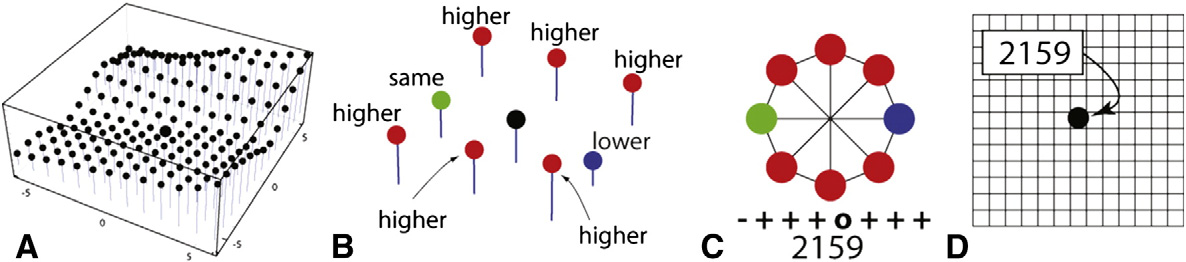
\includegraphics[width=0.75000\textwidth]{Geomorf3.png}
\caption{Modelo desarrollado por Jasiewicz \& Stepinski (2013) para la
caracterización del relieve.\label{Geomorf3}}
\end{figure}

\begin{figure}
\centering
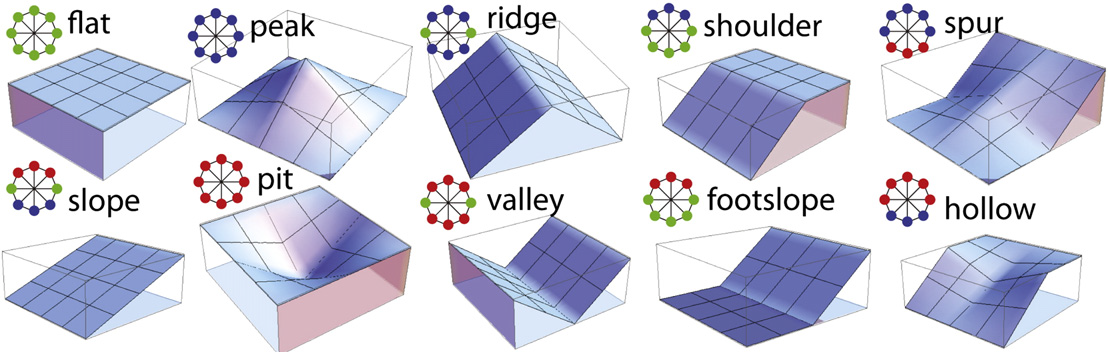
\includegraphics[width=0.75000\textwidth]{Geomor2.png}
\caption{Ejemplos de las variantes de relive más comunes obtenidas a
través del algoritmo (ibidem).\label{Geomorf2}}
\end{figure}

Diversos estudios fueron tomados en cuenta para la clasificación de
hábitats, se emplearon 5 de las categorías definidas por Harms, Condit,
Hubbell, \& Foster (2001) partiendo del resumen y análisis de la data
compilada en 16 años, donde fueron tomados en cuenta árboles iguales o
mayores de 1 cm de diámetro a la altura del pecho. (Ver tabla
\ref{tab:hábitat})

Table 2: Clasificación de hábitats, parcela permanente BCI (Harms et
al., 2001).\label{tab:hábitat}

\begin{longtable}[]{@{}lcc@{}}
\toprule
Hábitat & Pendiente (grados) & Elevación (metros)\tabularnewline
\midrule
\endhead
Bosque adulto - Meseta baja & \textless{}7 &
\textless{}152\tabularnewline
Bosque adulto - Meseta alta & \textless{}7 & = o
\textgreater{}152\tabularnewline
Bosque adulto - Pendiente & = o \textgreater{}7 & Todas\tabularnewline
Bosque adulto - Área pantanosa & Todas & Todas\tabularnewline
Bosque joven & Todas & Todas\tabularnewline
\bottomrule
\end{longtable}

Mapas de ubicación, abundancia de individuos, riqueza de especies,
agrupamiento de parcelas, pH, nitrógeno y otras variables presentes en
el relieve, clima, y edafología del lugar se emplearon para determinar
patrones asociativos entre las especies.

La determinación de la asociación interespecífica y de sitios muestrales
fue ralizada mediante los métodos R y Q respectivamente. El modo Q se
obtuvo con la métrica de distancia euclidea o similaridad de Jaccard,
verificando la paradoja de orlóci (1978); transformando la matriz en una
de cuerdas (\emph{chord}); \emph{ji}-cuadrado; y \emph{Hellinger}. A lu
vez, el modo R se calculó con el índice de correlación de Pearson
aplicando la transformación de \emph{chi} para corregir alteraciones
producidas por outliers en los datos, convirtiendo a binaria
(presencia/sencia) la matriz de comunidad transpuesta para calcular
distancias entre especies con la similaridad de Jaccard y el índice
\emph{rho} de Sperman. Por otro parte, el agrupamiento jerárquico fue
analizado mediante tres técnicas o criterios de enlace, donde fueron
seleccionados los criterios enlace simple y enlace promedrio de varianza
mínima tomando en cuenta métodos de regresión lineal {[}WARD{]}, siendo
la muestra dividida en tres grupos en este último. (Ver tabla
\ref{tab:enlace})

Table 3: Clasificación de los criterios de enlace (Harms et al.,
2001).\label{tab:enlace}

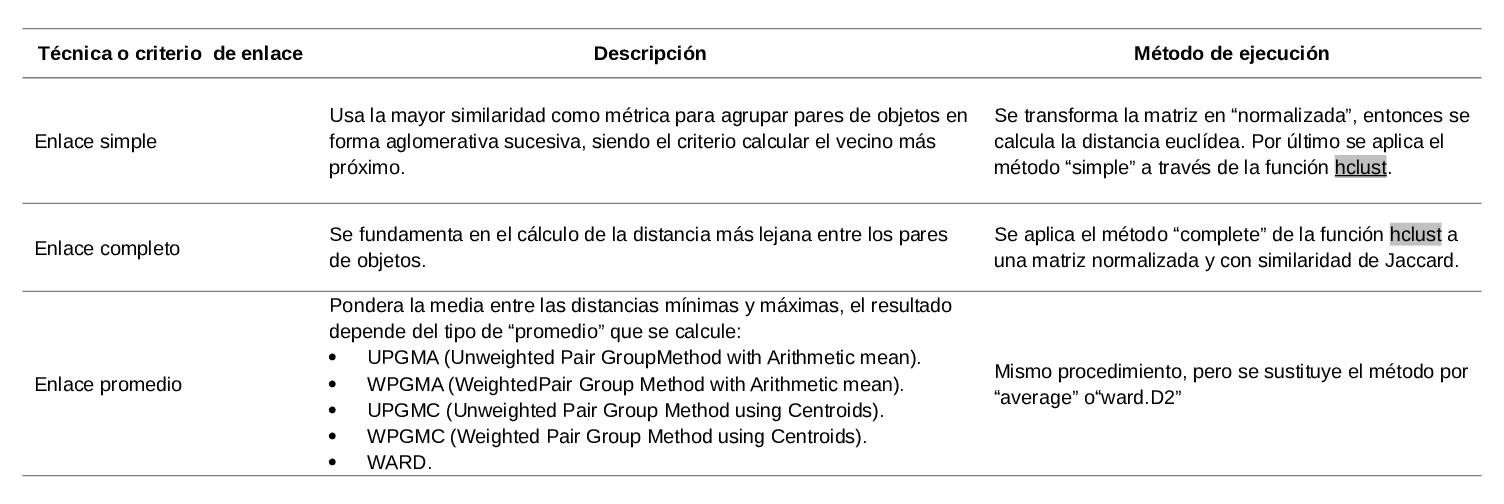
\includegraphics[width=1.00000\textwidth]{Análisis/Diversidad/Tabla_Criterios_Enlace.png}
\textbar{}

Se realizó una correlación entre los tres grupos determinados para WARD
y las variables ambientales para definir posibles asociaciones entre
estos o la exitencia de un grupo que se decante por al menos una
varibale en específico, fueron empleadas las pruebas ANOVA para evaluar
homogeneidad de medias y Kruskal-Wallis para evaluar homogeneidad de
medianas. De igual forma, fue generada la diversidad alpha aplicando la
función \emph{alpha\_div} a la matriz de comunidad, transformandola en
una matriz de índices, entropías, equidades y ratios. En específico se
crearon columnas con los índices N0 (Renyi), entropía H (diversidad de
Shannon), Hb2 (entropía de Shannon en base =2), los números de
diversidad de Hill (N1, Nb2, N2), J (equidad de Pielou), y las dos
ratios de Hill (E10 y E20).

Para obtner la estimación de riqueza de acuerdo a la diversidad de
especies en la parcela se emplearon los estimadores no paramétricos o de
``distribución libre'', entre estos están Chao1, Bootstrap, y los
Jackknife1 de primer y segundo orden.

\ldots

\section{Resultados}\label{resultados}

La parcela madre en BCI posee 3847 individuos de la familia
\emph{Fabaceae mimosoideae} agrupados en 18 especies distribuidas de
forma aleatoria en 50 sitios de 1ha cada uno. La especie más abundante
es \emph{Inga marginata} {[}767{]}, seguida de cerca por \emph{Inga
umbellifera} {[}765{]}; mientras que la más escasa es \emph{Cojoba
rufescens} {[}2{]}, seguida de \emph{Inga oerstediana} {[}4{]}. La
abundancia especifica acorde a una organización ascendente por número de
individuos presenta una mediana de 57 individuos {[}\emph{Inga punctata}
e \emph{Inga laurina}{]}, siendo la mitad más pobre de especies el
equivalente a un 5.82\% {[}224{]} y la mitad más presente el 94.18\%
{[}3623{]}. La riqueza de especies por cuadrante evidencia una
distribución también desproporcional, el C26 presenta la riqueza más
débil {[}5{]} y el C30 la más fuerte {[}13{]}. No obstante, aunque no
existe relación directa entre la riqueza y la abundancia por cuadrante,
en C26 coíncide y en algunos otros cuadros puede existir cierta
aproximación.

(ver tabla \ref{tab:abun_sp} y figura \ref{fig:abun_sp_q})

\begin{longtable}[]{@{}lr@{}}
\caption{\label{tab:abun_sp}Abundancia por especie de la familia
\emph{Fabaceae-Mimosoideae}.}\tabularnewline
\toprule
Latin & n\tabularnewline
\midrule
\endfirsthead
\toprule
Latin & n\tabularnewline
\midrule
\endhead
Inga marginata & 767\tabularnewline
Inga umbellifera & 765\tabularnewline
Inga acuminata & 606\tabularnewline
Inga nobilis & 557\tabularnewline
Inga goldmanii & 297\tabularnewline
Inga thibaudiana & 232\tabularnewline
Inga sapindoides & 197\tabularnewline
Inga pezizifera & 145\tabularnewline
Inga laurina & 57\tabularnewline
Inga punctata & 57\tabularnewline
Inga cocleensis & 54\tabularnewline
Acacia melanoceras & 48\tabularnewline
Inga spectabilis & 20\tabularnewline
Abarema macradenia & 19\tabularnewline
Enterolobium schomburgkii & 12\tabularnewline
Inga ruiziana & 8\tabularnewline
Inga oerstediana & 4\tabularnewline
Cojoba rufescens & 2\tabularnewline
\bottomrule
\end{longtable}

\begin{figure}
\centering
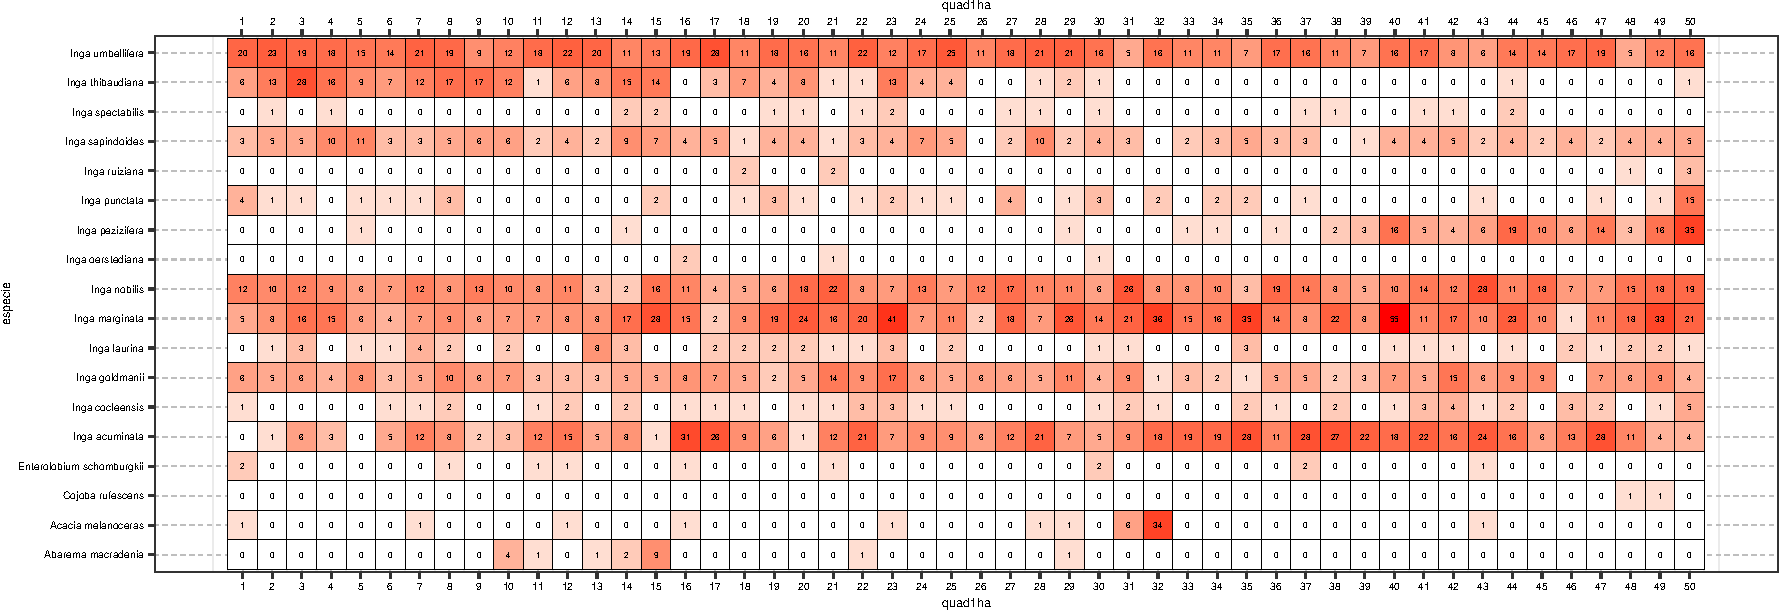
\includegraphics{manuscrito_files/figure-latex/unnamed-chunk-3-1.pdf}
\caption{\label{fig:abun_sp_q}Abundancia por especie por quadrat}
\end{figure}

El terreno eminentemente describe una geomorfología en vertiente, siendo
esta característica la más destacada en el 88\% de los C 1Ha; en tanto
que el 12\% restante describe una geomorfología donde predomina el
relieve llano. La parcela madre está compuesta en un 52\% por bosque
adulto en meseta baja distribuido ampliamente, un 24\% por bosque adulto
en pendiente con presencia marcada en las parcelas {[}C41-C45{]}, un
16\% por bosque adulto en meseta alta concentrado en las parcelas
{[}C32-C34; C37-C40{]}, mientras que el 8\% restante es hábitat
pantanoso y bosque jovén en forma equitativa. No parece existir una
relación directa entre la morfología del espacio y un determinado
hábitat, exeptuando el bosque joven que se encuentra tanto en llanura
como en vertiente de forma considerable. En general, se percibe un leve
aumento de la riqueza específica a medida que aumenta la abundancia de
individuos; destacando la abundante riqueza de especies en el hábitat
pantanoso, su pobreza en el bosque adulto en zona alta, la abundancia
marcada el bosque adulto en zona baja y su riqueza equilibrada . (Ver
figura \ref{fig:leal}).

\begin{figure}
\centering
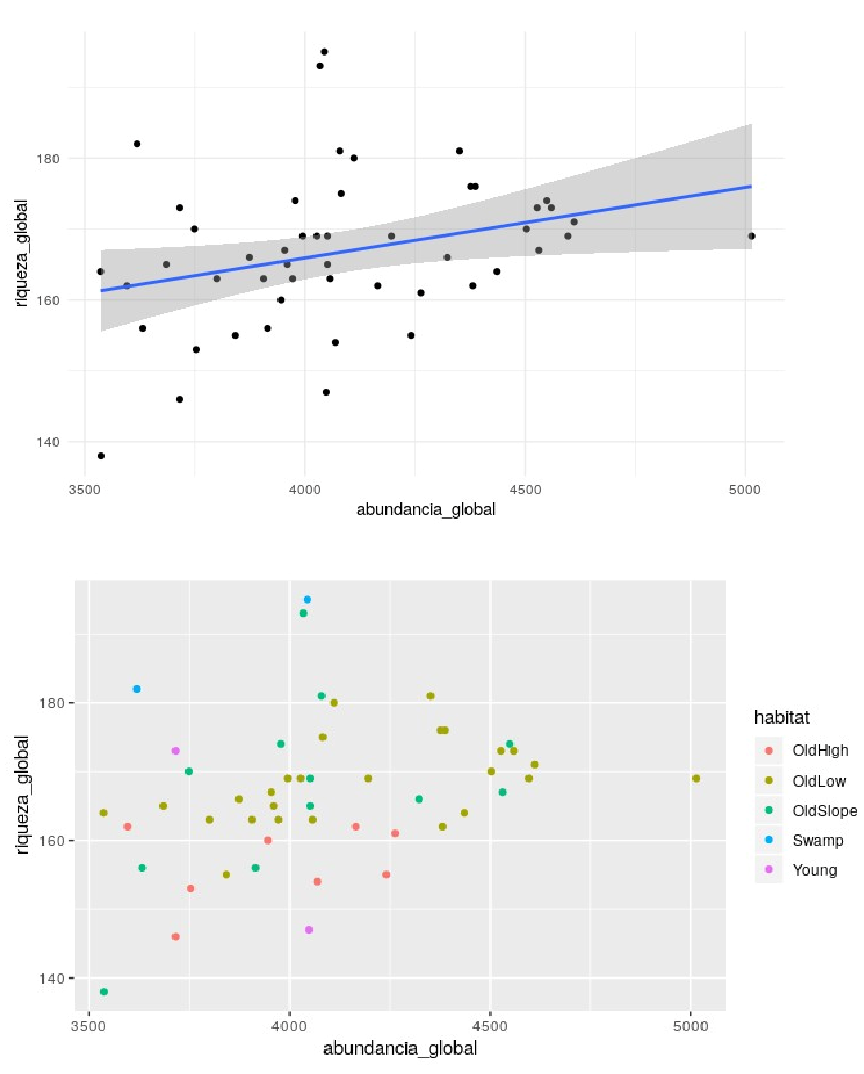
\includegraphics[width=1.00000\textwidth]{Análisis/Diversidad/Graf_regre_lineal_aed_2.png}
\caption{Distribución de sitios en función de su riqueza, abundancia, y
hábitat dominante.\label{fig:leal}}
\end{figure}

El grado de asociación según la similaridad de Jaccard acorde a la
abundancia de especies por cuadro con matriz transformada
\emph{Hellinger} expone la existencia de clústers super semejantes
limitados por los sitios C28-C33; C33-C40; C24-C2; C8-C10. Estos sitios
comparten un 75\% o más de las especies de acuerdo con la matriz
ordenada en función de la relación de proximidad (ver mapa de calor
superior \ref{fig:heat}). Por otra parte, la presencia de variables
edáficas como minerales y otros elementos está asociada a la abundancia
de especies en el clúster formado por los sitios C1-C9 de la matriz
ordenada en función del id de lugar, pero además de esta relación no hay
indicios de una dependencia entre estas variables que evidencie
asociación alguna (ver mapa de calor inferior \ref{fig:heat}). De igual
forma, no existe una relación de asociación entre las variables mixtas
``hábitat, quebrada, heterogeneidad ambiental'' y la distribución de
especies por cuadros. (Ver figura \textbackslash{}ref\{fig:heat).

\begin{figure}
\centering
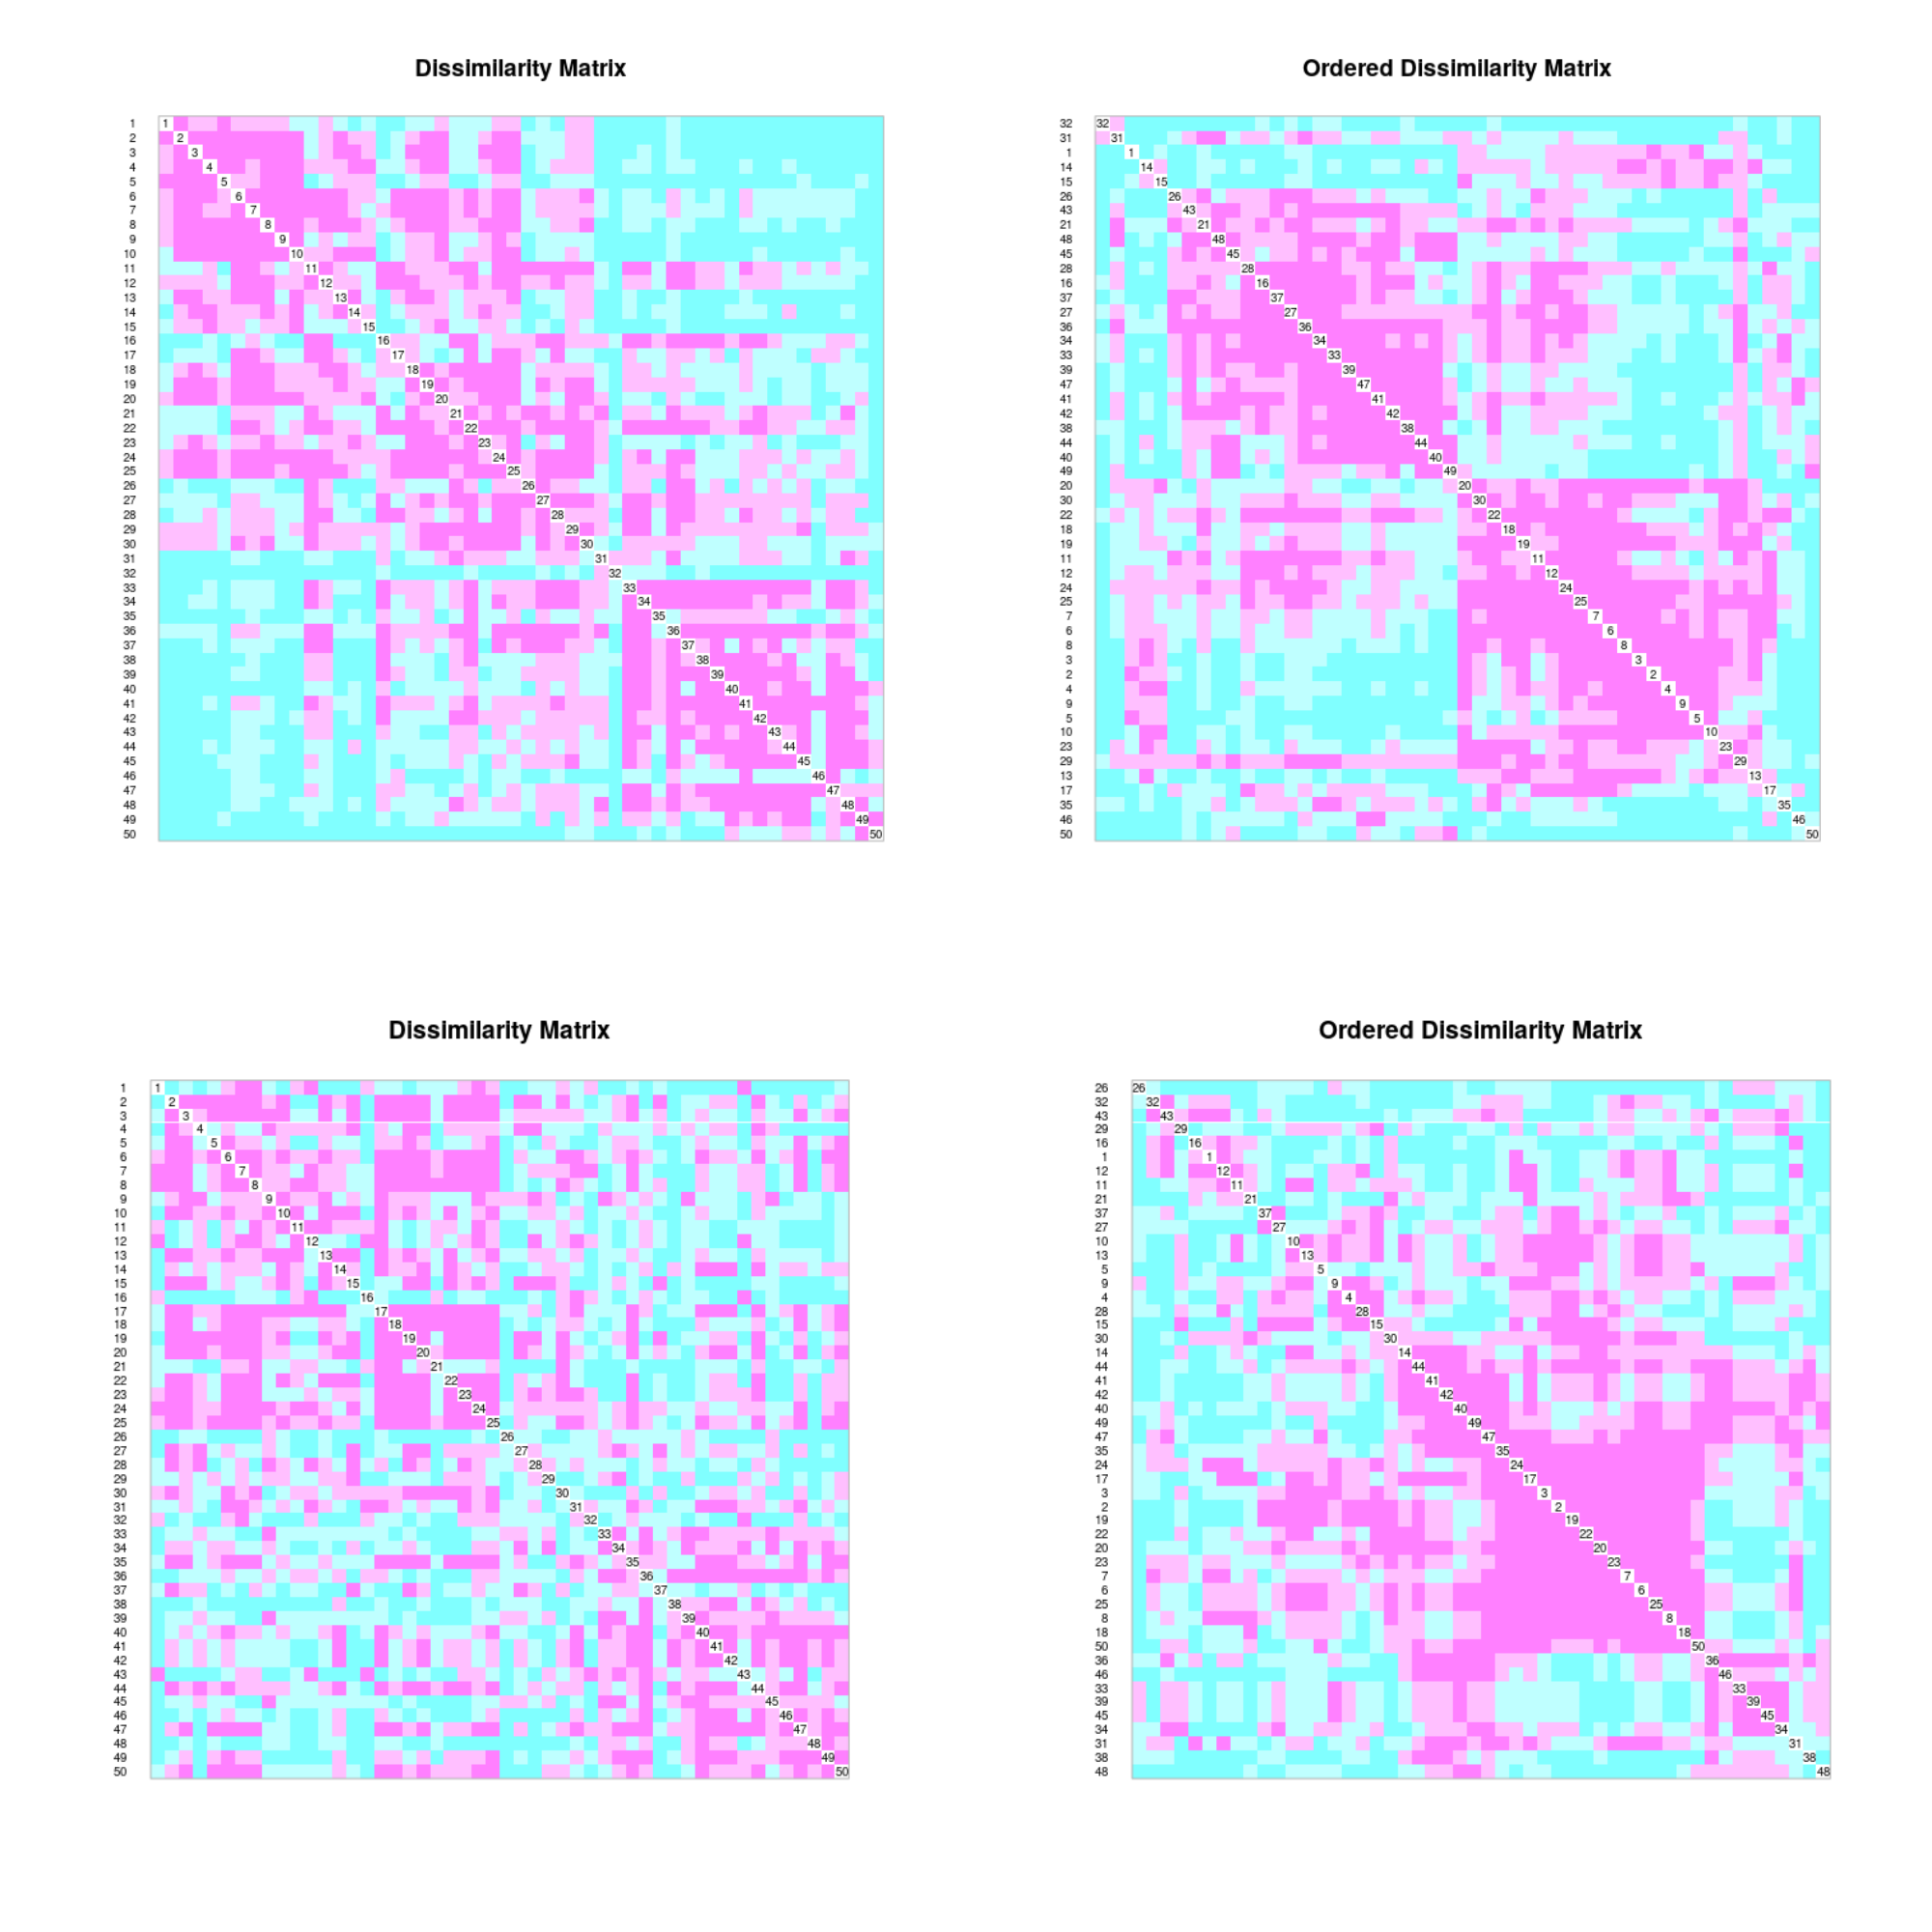
\includegraphics[width=0.50000\textwidth]{Análisis/Imágenes manuscrito/Heat_maps_Q.png}
\caption{Mapas asociación de especies por abundancia en los sitios de
muestreo (superior) y por asociación de variables ambientales y
abundancia (inferior). El color azul fuerte representa ``lejanía'' y el
rosado fuerte ``proximidad''.\label{fig:heat}}
\end{figure}

La asociación interespecífica en función de la abundancia, como se
observa en el mapa de calor \ref{fig:heat1}, evidencia un grado de
asociación muy amplio {[}75\%-100\%{]} en el clúster delimitado por
\emph{Inga lauriana} e \emph{Inga margitana}, así como uno considerable
en el macroclúster comprendido entre \emph{Inga pezizifera} e \emph{Inga
spectabilis}. Es descrito un patrón similar por las especies en la
matriz binaria (presencia/ausencia), donde se forma un clúster entre
\emph{Inga cocleensis} e \emph{Inga laurina} que describe bastante
coexistencia entre las especies {[}75\%-100\%{]}, y un macroclúster
entre \emph{Inga pezizifera} e \emph{Inga spectabilis} con cercanía
considerable. En ese sentido, la matriz de correlación entre las
variables ``abundancia, riqueza, y composición del suelo'' ,realizada
mediante el índice \emph{rho} de sperman, corrobora lo observado en los
mapas de calor anteriores acerca del escaso grado de asosiación entre
dichas variables. Tampoco se observa relación entre las dos primeras y
las variables relativas a la geomorfología del lugar. (Ver figura
\ref{fig:sper})

\begin{figure}
\centering
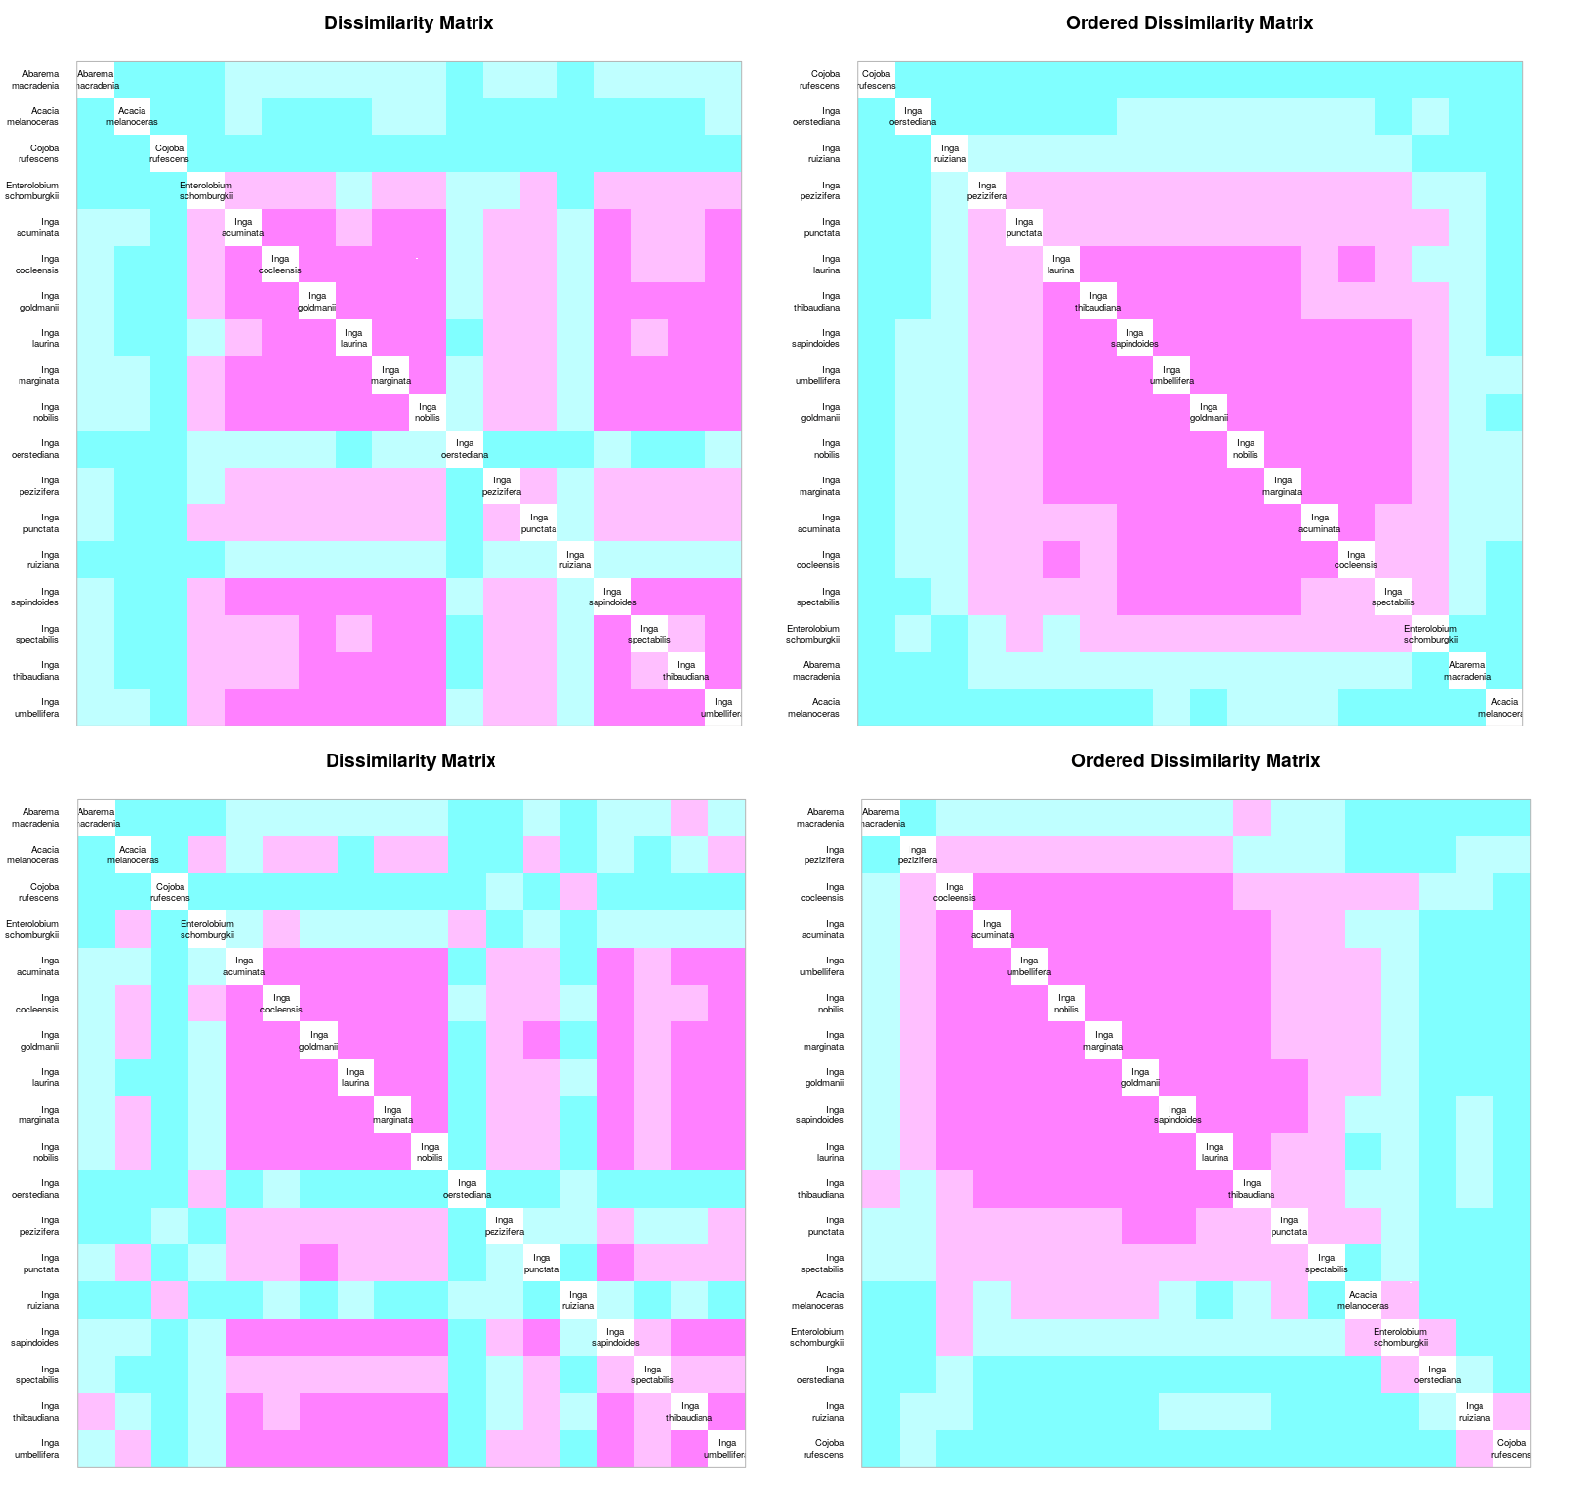
\includegraphics[width=1.00000\textwidth]{Análisis/Imágenes manuscrito/Heat_Map_R.png}
\caption{Mapas de calor, asociación entre especies en función de su
abundancia (superior)y en función de su abundancia con matríz binaria
``presencia/ausencia'' (inferior).\label{fig:heat1}}
\end{figure}

\begin{figure}
\centering
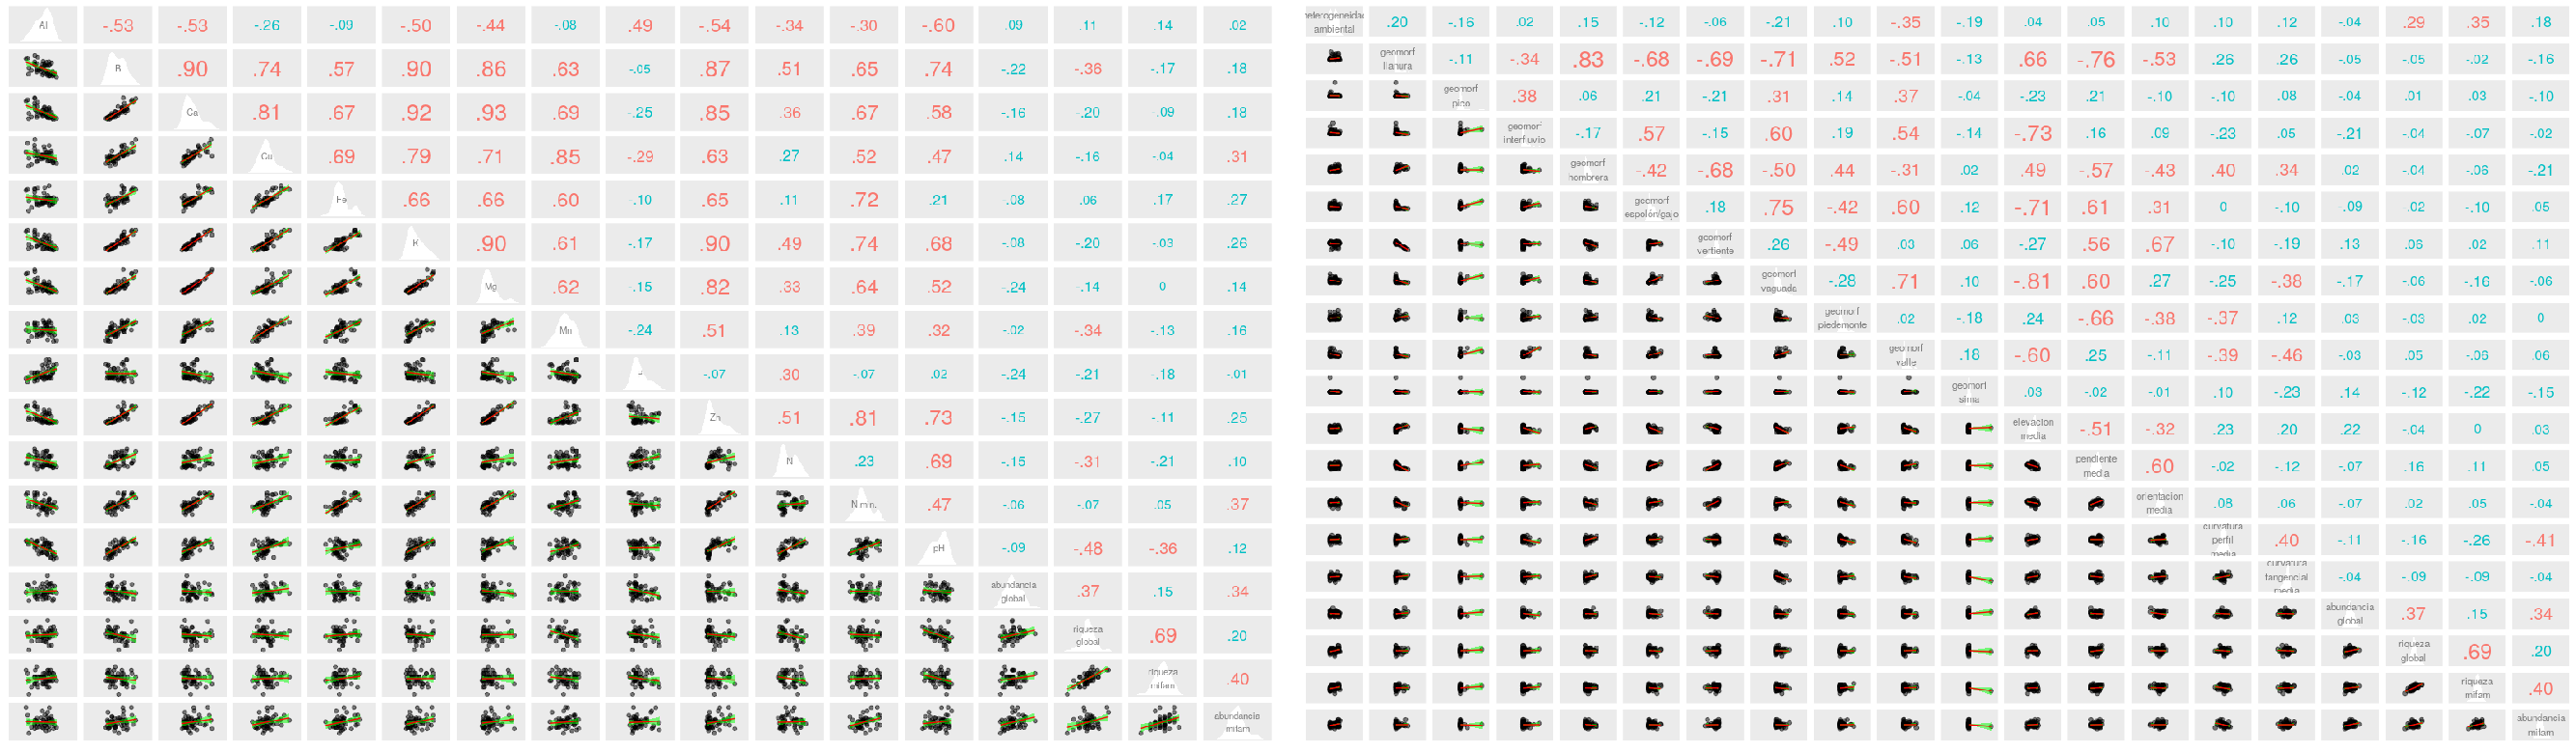
\includegraphics[width=1.00000\textwidth]{Análisis/Imágenes manuscrito/Seperman_R.png}
\caption{Matrices de Sperman, asociación de especies en función de las
variables edáficas (superior) y asociación de especies en función de las
variables geomorfológicas (inferior) .\label{fig:sper}}
\end{figure}

Acorde al ordenamiento por enlace simple, los cuadros 32, 50 y 43 se
separan bastante de los demás, lo cual se corresponde con la abundancia
y riqueza de especies en estos sitios comparada con los demás, siendo en
C32 116 {[}tercera más alta{]} y 8 {[}tercil más pobre{]}
respectivamente, por ejemplo. También se observan dos grupos definidos
formados entre los sitios C22-C37 y C28-C7. (Ver \label{fig:denS})

\begin{figure}
\centering
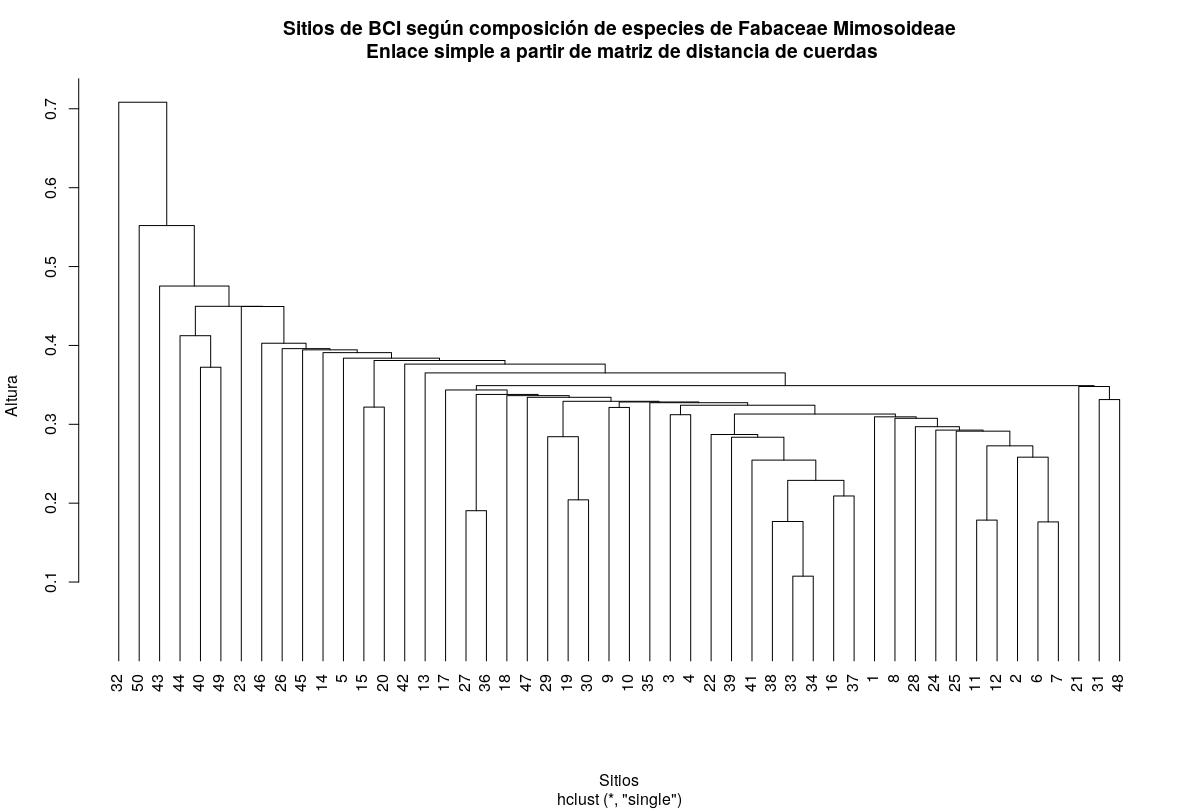
\includegraphics[width=1.00000\textwidth]{DenSimple.png}
\caption{Dendrograma a partir del criterio enlace
simple.\label{fig:denS}}
\end{figure}

En el dendrograma de WARD se observa la presencia de de tres grupos
definidos entre los sitios C3-C7, C46-C34 y C27-C23; formados por 11, 18
y 21 sitios respectivamente. También pueden definirse cinco subgrupos
menores más próximos entre sí: C3-C7 {[}sitios con abundacia y riqueza
promedio{]}, C46-C22, C27-C48, C50-C23 {[}citios con las mayores
abundancias y riquezas, o al menos una de estas en forma de outlier{]}
(ver figura\ref{fig:denW}).Continuando con los tres primeros grupos WARD
mencionados, en los diagramas de cajas para las variables ambientales se
observa distancia que se acrecenta según se cambia de grupo, en orden
ascendente, en las medianas respecto a las variables Boro, Hierro,
Geomorfología en llanura, Potasio, Nitrógeno Minimo, pH y zinc.Esta
tendencia es también descrita en menor medida por las variables Calcio,
Cobre, Heterogeneidad ambiental y Magnesio. En constrate, este patrón se
invierte en las variables Aluminio y Geomorfología en vaguada. Por otra
parte, el segúndo grupo se decanta por la variable Fósforo, presentando
números inferiores en Abundancia y Riqueza de especies, mientras que el
primer y tercer grupo son bastante homogéneos en ese sentido.

\begin{figure}
\centering
\includegraphics[width=1.00000\textwidth]{Inter_Ward_5Clústers_Dendrogram.png}
\caption{Dendrograma a partir del criterio enlace promedio
(WARD).\label{fig:denW}}
\end{figure}

\begin{figure}
\centering
\includegraphics[width=1.00000\textwidth]{WARD_Plots_Variables_Ambientales_Clústers.png}
\caption{Diagramas de cajas en función de las variables ambientales para
los grupos WARD.\label{fig:boxW}}
\end{figure}

En la matriz de correlación para determinar equidad se observan niveles
de correlación bastante bajos para todas la variables ambientales,
siendo las variables Boro, Fósforo, Nitrógeno y pH las que presentan
niveles significativos respecto a los números de Hill y los índices de
Shannon. Por otra parte, la variable ``Riqueza global'' presenta niveles
determinantes para los índices anteriores, promediando un 73\% de
correlación colectivamente.

\begin{figure}
\centering
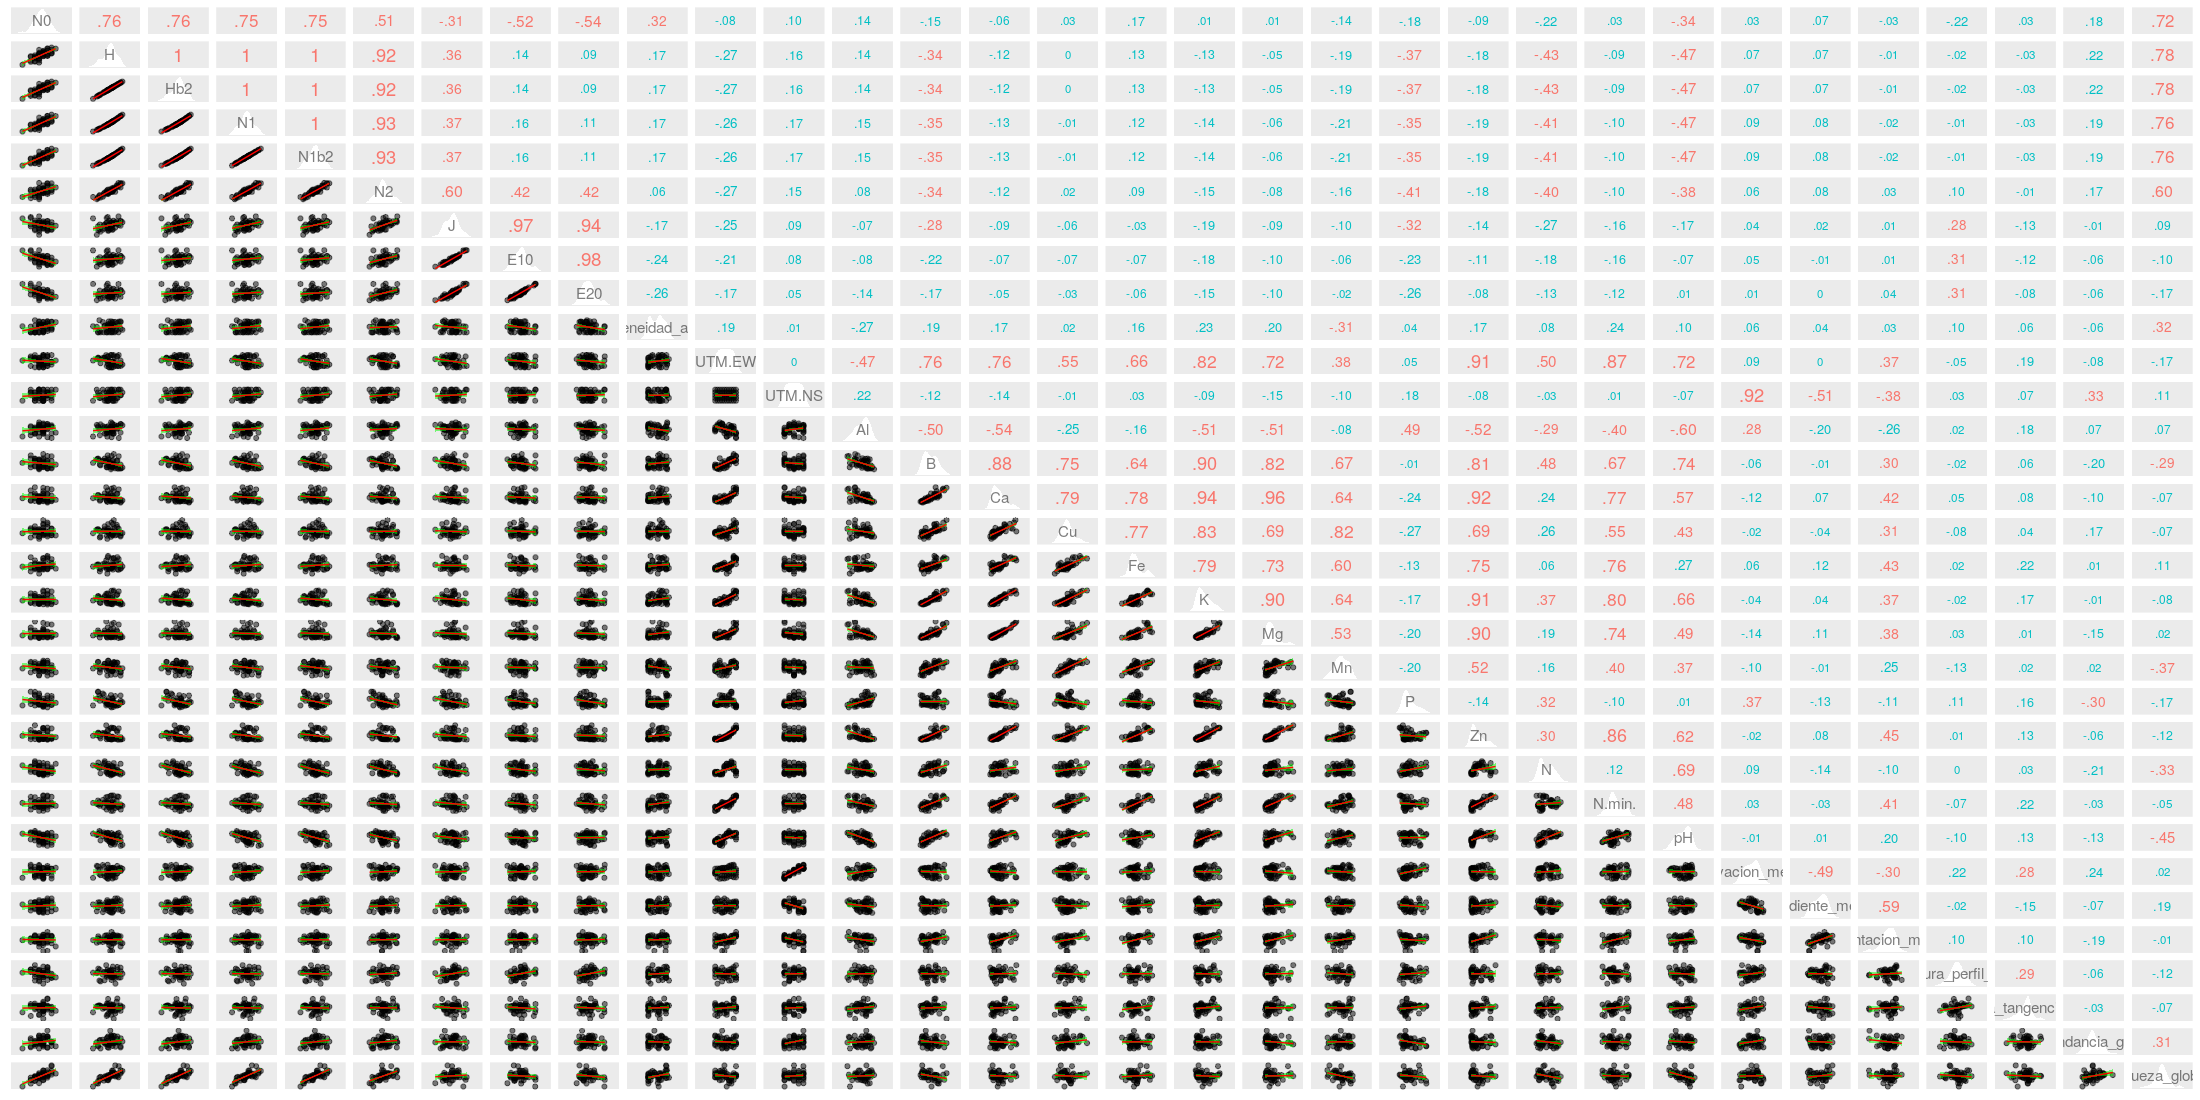
\includegraphics[width=1.00000\textwidth]{Análisis/Diversidad/Índices_Env_Diversidad_Alpha_2.png}
\caption{Matriz de diversidad alpha: correlación entre indices,
entropías, equidades, y ratios con las variables
ambientales.\label{fig:divA}}
\end{figure}

\textbf{\emph{Insertar matriz 2, análisis diversidad alpha}}

La riqueza de especies respecto a la diversidad de estas en la parcela
se determinó en porcentajes aproximados a la riqueza real. Por otro
lado, la diversidad beta describe una curva ascendente según aumenta el
número de ordenamiento en Hill, llegando a superar el N0. Presentando un
grado de dominancia mayor y una dependencia de la abundancia en la
diversidad beta. Las especiees que más contribuen a la diversidad son
\emph{Inga acumiata}, \emph{Inga marginata}, \emph{Inga Pezizifera} e
\emph{Inga thibaudiana}; donde las dos primeras son de las especies más
abundantes y por si solas representan el 35.7\% de los individuos en la
comunidad de las fabaceas. Por otra parte, los sitios que más
contribuyen a la diversidad beta son C32 y C50. (Ver tabla
\ref{tab:est})

Table 4: Estimadores de riqueza de especies. \label{tab:est}

\begin{longtable}[]{@{}llllll@{}}
\toprule
Estimadores & Chao & Jackknife1 & Jackknife2 & Bootstrap &
Real\tabularnewline
\midrule
\endhead
& 18 (100\%) & 18 (100\%) & 17.06 (105.5\%) & 18.19 (98.95\%) &
18\tabularnewline
\bottomrule
\end{longtable}

\section{Discusión}\label{discusiuxf3n}

La familia \emph{Fabaceae mimosoideae} en BCI presenta niveles de
asociación (coexistencia) sobre el 75\% entre las especies \emph{Inga
laurina}, \emph{Inga margitana}, \emph{Inga thitaudiana}, \emph{Inga
sapindoides}, \emph{Inga umbellifera}, \emph{Inga goldimanii} e
\emph{Inga nobilis}. Estas especies son las más abundantes de esta
familia e BCI, exceptuando por \emph{Inga laurina} que tomando en cuenta
sus apenas 57 individuos se encuentra ampliamente distribuida. Ninguna
variable ambiental resultó determinante en la existencia de especies en
los cuadros, aunque existen relaciones significativas entre las
variables edáficas Al {[}grupo 1{]}, K {[}grupo 2{]}, pH y Zn {[}grupo
3{]}.

La composición de las fabaceas es bastante uniforme tomando en cuenta
que a través del criterio de enlace promedio UPGMA no se pudo dividir
las muestras de forma efectiva en dos grupos {[}resultando en 49 y 1{]}.
Sin embargo, mediante el método promedio de la varianza mínima se pudo
separar efectivamente la muestra en tres grupos de cuadros, los cuales
presentaron medianas bastante aproximadas entre si para la mayoría de
variables ambientales.

La diversidad de las especies no esta afectada de forma significativa
por alguna variable, siendo la equidad poco signifcativa para todas las
variables ambientales, exceptuando por la abundancia globadl que es la
determinante de la diversidad en la muestra. En ese sentido, la riqueza
las fabaceas respecto a la diversida es bastante alta, teniendo
porcentajes mayores al 98\% en todos los índices calculados. Cuatro
especies contribuyen significativamente a la dversidad: \emph{Inga
marginata}, \emph{Inga acumiata}, \emph{Inga thibaudiana} e \emph{Inga
Pezizifera}, todas ellas pertenecientes a la mitad mas abundante de las
especies.

\section{Agradecimientos}\label{agradecimientos}

Este trabajo fue posible gracias al Ph.D José Ramón Martinez Battle,
quien supervisó todo el proceso, brindó la asesoría y fuentes
bibliográficas de partida. Sin él este trabajo nose habría realizado.

\section{Información de soporte}\label{informaciuxf3n-de-soporte}

\ldots

\section{\texorpdfstring{\emph{Script}
reproducible}{Script reproducible}}\label{script-reproducible}

\ldots

\hypertarget{refs}{}
\hypertarget{ref-inproceedings}{}
Baldeck, C., Asner, G., Martin, R., Anderson, C., Knapp, D., Kellner,
J., \& Wright, S. J. (2014). Operational tree species mapping in a
diverse tropical forest with airborne imaging spectroscopy. \emph{PloS
one}, \emph{10}. \url{https://doi.org/10.1371/journal.pone.0118403}

\hypertarget{ref-jose_ramon_martinez_batlle_2020_4402362}{}
Batlle, J. R. M. (2020). biogeografia-master/scripts-de-analisis-BCI:
Long coding sessions (Version v0.0.0.9000).
\url{https://doi.org/10.5281/zenodo.4402362}

\hypertarget{ref-condit1998tropical}{}
Condit, R. (1998). \emph{Tropical forest census plots: Methods and
results from barro colorado island, panama and a comparison with other
plots}. Springer Science \& Business Media.

\hypertarget{ref-condit1999dynamics}{}
Condit, R., Ashton, P. S., Manokaran, N., LaFrankie, J. V., Hubbell, S.
P., \& Foster, R. B. (1999). Dynamics of the forest communities at pasoh
and barro colorado: Comparing two 50--ha plots. \emph{Philosophical
Transactions of the Royal Society of London. Series B: Biological
Sciences}, \emph{354}(1391), 1739--1748.

\hypertarget{ref-harms2001habitat}{}
Harms, K. E., Condit, R., Hubbell, S. P., \& Foster, R. B. (2001).
Habitat associations of trees and shrubs in a 50-ha neotropical forest
plot. \emph{Journal of Ecology}, \emph{89}(6), 947--959.

\hypertarget{ref-hasanuzzaman2020plant}{}
Hasanuzzaman, M., Araújo, S., \& Gill, S. S. (2020). \emph{The plant
family fabaceae: Biology and physiological responses to environmental
stresses}. Springer Nature.

\hypertarget{ref-jasiewicz2013geomorphons}{}
Jasiewicz, J., \& Stepinski, T. F. (2013). Geomorphons---a pattern
recognition approach to classification and mapping of landforms.
\emph{Geomorphology}, \emph{182}, 147--156.

\hypertarget{ref-montagnini2005tropical}{}
Montagnini, F., Jordan, C. F., \& others. (2005). \emph{Tropical forest
ecology: The basis for conservation and management}. Springer Science \&
Business Media.

\hypertarget{ref-Moreno2001}{}
Moreno, C. (2001). \emph{Métodos para medir la biodiversidad} (Vol. 1).

\hypertarget{ref-saikia2020tropical}{}
Saikia, P., Nag, A., Anurag, S., Chatterjee, S., \& Khan, M. L. (2020).
Tropical legumes: Status, distribution, biology and importance. In
\emph{The plant family fabaceae} (pp. 27--41). Springer.

\hypertarget{ref-venables2009introduction}{}
Venables, W. N., Smith, D. M., Team, R. D. C., \& others. (2009).
\emph{An introduction to r}. Citeseer.




\newpage
\singlespacing 
\end{document}
